\documentclass{article}
\usepackage[margin=1in]{geometry}
\usepackage{graphicx}
\usepackage{amsmath}
\usepackage{booktabs}
\usepackage{placeins}
\usepackage[hypertexnames=false]{hyperref}
\renewcommand{\figurename}{Fig.}

% results/ is the overleaf-synced folder; diagnostics/ (formerly
% v1_v2_comparison/) holds the pipeline-validation figures.
\graphicspath{{results/}{diagnostics/}{v1_v2_comparison/}{plots/}}

\title{Calibration results:\\
MCMC inference of subgrid + cosmology parameters \\ (in Progress)}
\author{}
\date{}

\begin{document}
\maketitle

\section{Setup}

The likelihood combines emulator predictions with published
observations, summed over the requested observables:
\begin{equation}
\ln\mathcal{L}(\theta) = -\tfrac{1}{2}\sum_{o\in \mathrm{obs}}
\sum_{i} \frac{(y^{\rm obs}_{o,i} - \mu^{\rm emu}_o(\theta;x_i))^2}
              {\sigma^{\rm obs\,2}_{o,i}}.
\end{equation}
Sampling uses \texttt{emcee} with 400 walkers, 100 burn-in steps, 4000
production steps and parallel evaluation, over the 109-point Latin-hypercube
design (\texttt{FinalDesign.txt}; 5 subgrid $+$ 2 cosmology parameters,
$400\,h^{-1}{\rm Mpc}$ HAvoCC boxes). Subgrid priors are Gaussian, centred
at the design midpoint with $\sigma=$ half the design range, except
$\epsilon_{\rm kin}$ (index 4), which is flat. Walkers are initialised
uniformly across each parameter's design range.

\paragraph{Cosmology prior (Planck-width, \texttt{*\_pk}).} This update adopts a
\emph{Planck-informed} cosmology prior for all cosmology-varying runs: a Gaussian
centred at the project fiducial with $\sigma_{\omega_m}=0.0011$ and
$\sigma_{\sigma_8}=0.006$, bounded only by the design box (\emph{no} hard cut).
These are the \texttt{*\_pk} configurations, and they are now the canonical
cosmology fits (see \S\ref{sec:cosmo}). The earlier moderate-width prior
($\sigma_{\omega_m}=0.005$, $\sigma_{\sigma_8}=0.03$) let the fixed-hydro
likelihood rail the posterior to the design-box edges; the retired moderate-prior
chains live under \texttt{old\_results/retired\_moderate\_prior/}.

\paragraph{Project fiducial cosmology.} When cosmology is fixed
(\texttt{param\_mode: subgrid}), the values used are
$\omega_{\rm m}\!\equiv\!\Omega_m h^2=0.14176$ and $\sigma_8=0.8102$
(from $\Omega_{\rm cdm}=0.26067$, $\Omega_b h^2=0.02242$, $H_0=67.66$,
$n_s=0.9665$). The fiducial subgrid point is
$(\kappa_{\rm w}, e_{\rm w}, M_{\rm seed}/10^6, v_{\rm kin}/10^4,
\epsilon_{\rm kin}/10^1) = (3,\,0.5,\,0.8,\,0.51,\,0.13)$.

\paragraph{Trials.} Configurations live in
\texttt{Inference/configs/} and are deep-merged on top of
\texttt{\_defaults.yaml}. Headline trials:
\begin{itemize}
  \item \texttt{GSMF\_5p\_fid\_cosmo}: GSMF only, cosmology fixed, 5
        subgrid parameters free.
  \item \texttt{GSMF\_7p\_pk}: GSMF only, all 7 parameters free, Planck
        cosmology prior.
  \item \texttt{GSMF\_CGD\_7p\_pk}: GSMF $+$ cluster gas density (CGD)
        joint calibration, all 7 parameters free, Planck cosmology prior.
  \item \texttt{GSMF\_\{2cosmo\}\_pk}, \texttt{GSMF\_CGD\_2cosmo\_pk}:
        cosmology-only fits with hydro fixed at fiducial (control for the
        marginalization test).
  \item \texttt{CGD\_CGED\_cluster}: cluster-only fit, cosmology fixed.
\end{itemize}

\FloatBarrier

\section{GSMF and GSMF$+$CGD headline fits with posterior-predictive summaries}

Each MCMC fit is shown together with its \emph{posterior-predictive summary}:
the emulator prediction evaluated at the best-fit (GMM mode) parameters, overlaid
on the observations, with a shaded 90\% band from the emulator's analytic
variance. The parameter modes are printed in the coloured textbox.

\begin{figure}[htbp]
    \centering
    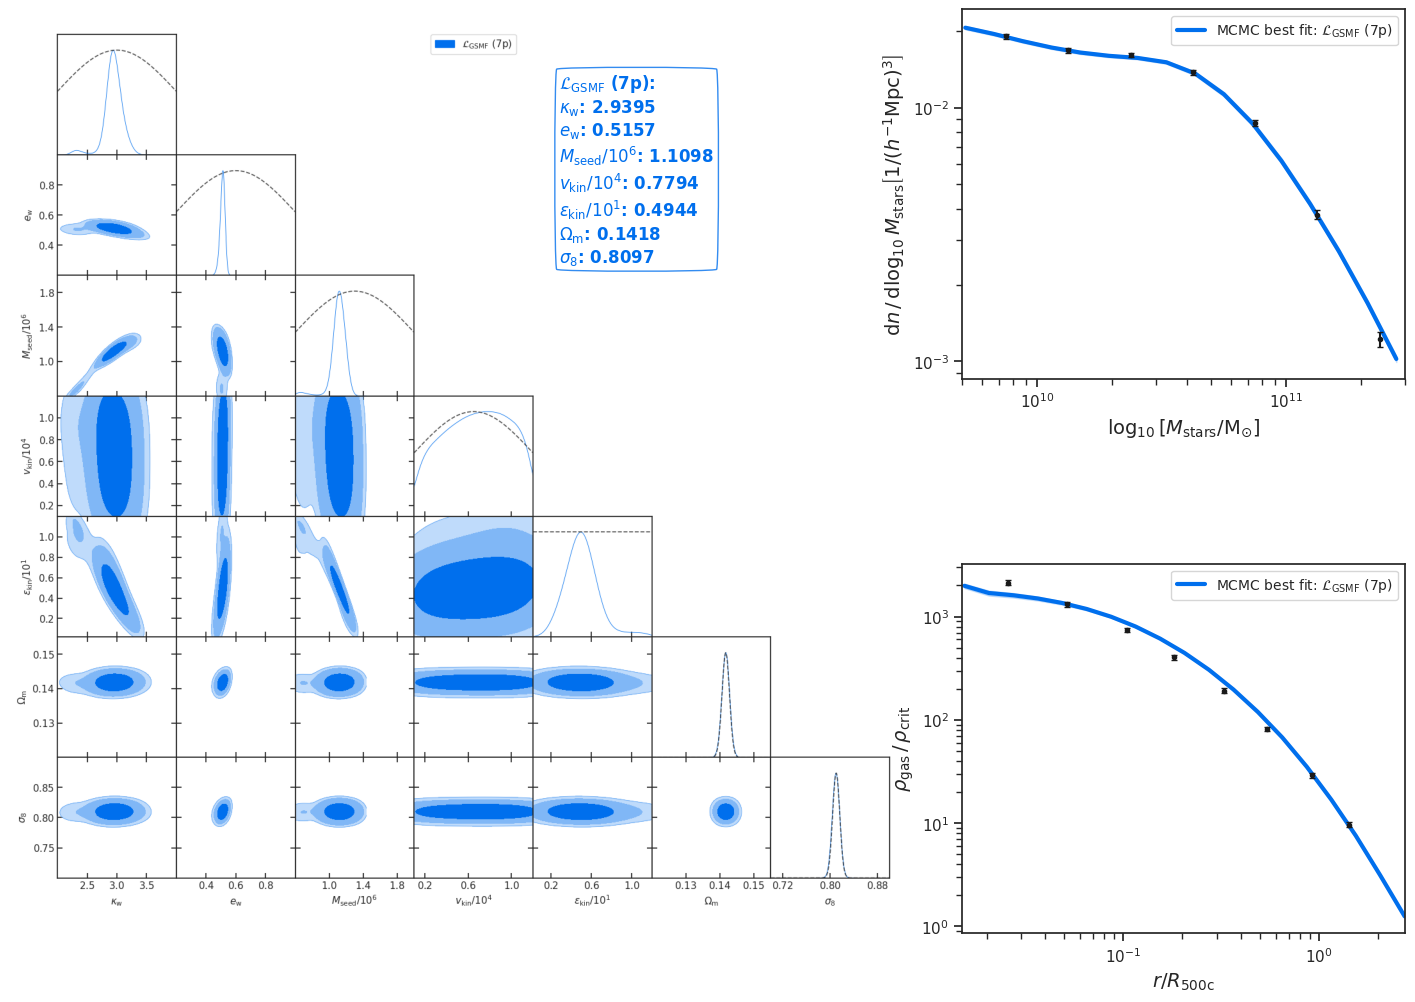
\includegraphics[width=1\linewidth]{plot_summary_GSMF_7p_planck.png}
    \caption{\texttt{GSMF\_7p\_pk}: seven-parameter posterior (5 subgrid $+$ 2
    cosmology) from the GSMF emulator under the Planck cosmology prior, with the
    best-fit GSMF (and predicted CGD) overlaid on the data (right). The GSMF
    amplitude and slope are reproduced across the full stellar-mass range. GSMF
    alone constrains $\sigma_8$ through the high-mass tail but leaves the kinetic
    feedback parameters ($v_{\rm kin}, \epsilon_{\rm kin}$) broad.}
    \label{fig:summary_gsmf}
\end{figure}

\begin{figure}[htbp]
    \centering
    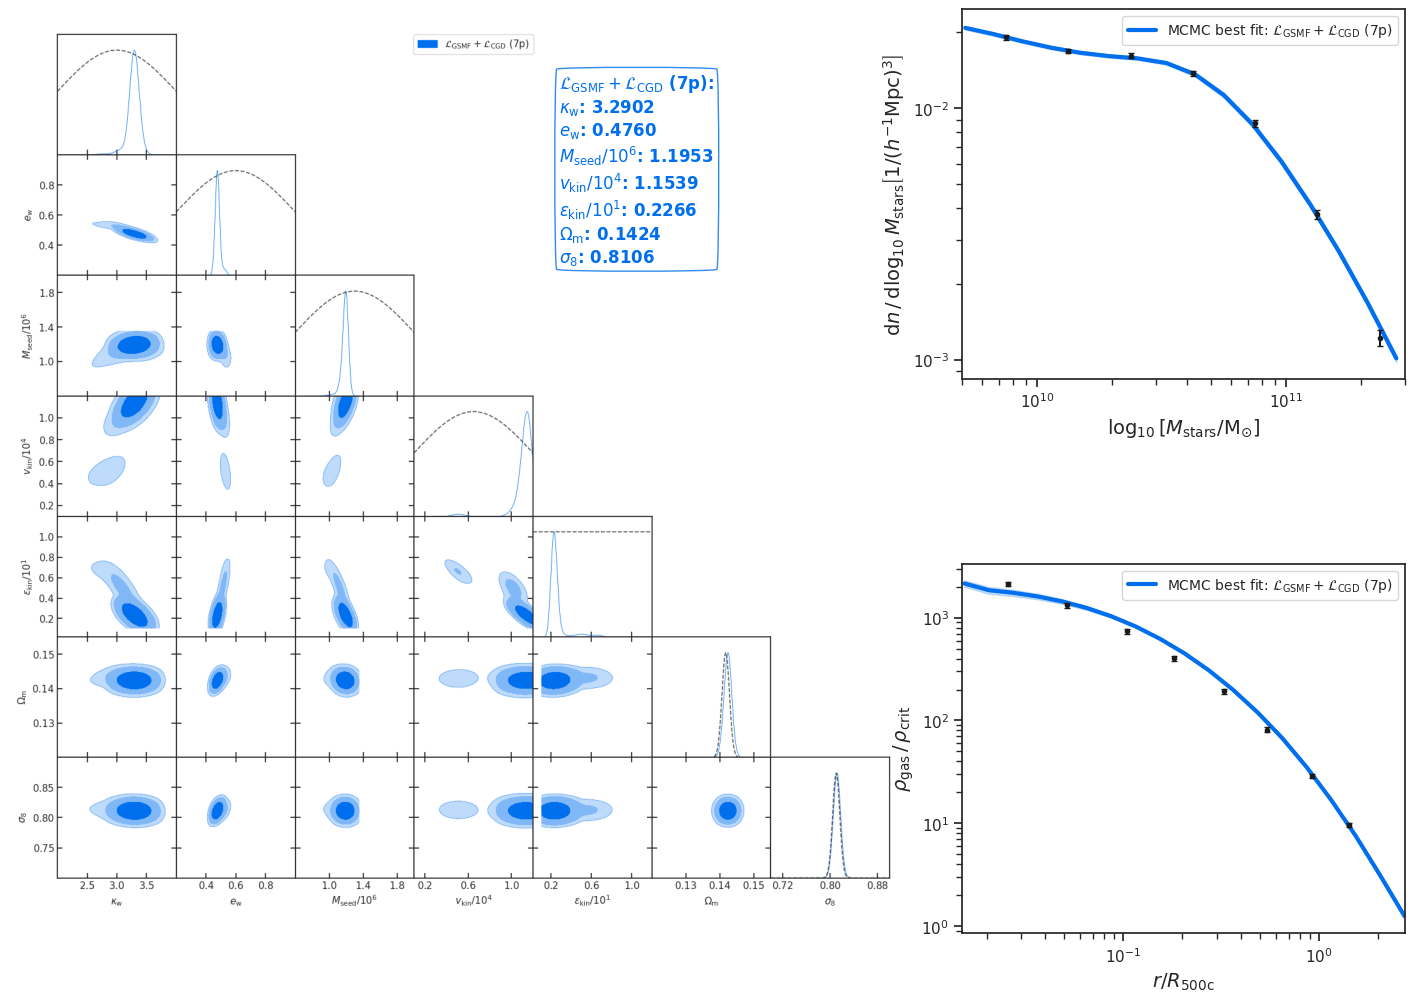
\includegraphics[width=1\linewidth]{plot_summary_GSMF_CGD_7p_planck.png}
    \caption{\texttt{GSMF\_CGD\_7p\_pk}: same, for the GSMF$+$CGD joint fit.
    Both the GSMF and the cluster gas-density profile are reproduced within the
    observational errors; the CGD only slightly underpredicts the innermost
    radial bin. Adding CGD sharply tightens $\kappa_{\rm w}$, $v_{\rm kin}$ and
    $\epsilon_{\rm kin}$ relative to GSMF alone.}
    \label{fig:summary_gsmf_cgd}
\end{figure}

\begin{figure}[htbp]
    \centering
    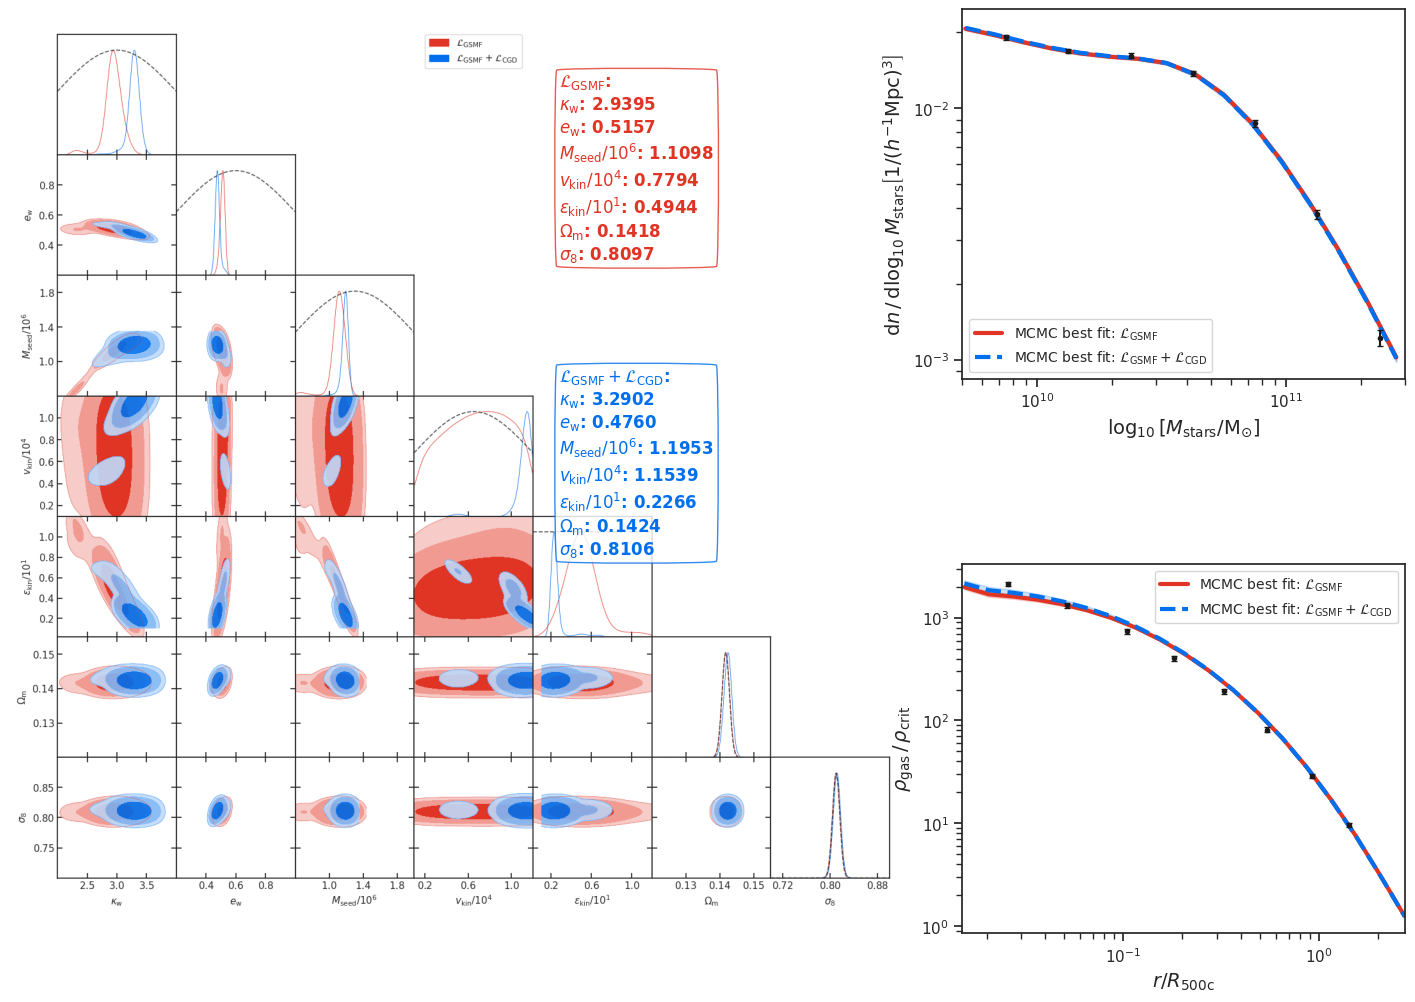
\includegraphics[width=1\linewidth]{plot_summary_7p_GSMF_vs_GSMF_CGD_planck.png}
    \caption{Direct overlay of \texttt{GSMF\_7p\_pk} (red) and
    \texttt{GSMF\_CGD\_7p\_pk} (blue). The two forward models give
    statistically indistinguishable GSMF predictions (top-right) despite reaching
    different feedback parameters, confirming the GSMF is degenerate in the
    kinetic-feedback sector. CGD breaks that degeneracy: the joint fit collapses
    $v_{\rm kin}$ and $\epsilon_{\rm kin}$ onto tight modes. Both fits agree on
    cosmology ($\omega_m\!\approx\!0.142$, $\sigma_8\!\approx\!0.81$).}
    \label{fig:summary_compare}
\end{figure}

\FloatBarrier

\section{Cosmology: marginalizing vs.\ fixing, and the Planck prior}
\label{sec:cosmo}

\paragraph{Why weak cosmology priors railed.} When hydro is \emph{fixed} at
fiducial and only $(\omega_m, \sigma_8)$ vary, the hydro$\leftrightarrow$cosmology
degeneracy is broken and the resulting likelihood is steep: it dominates any weak
prior and pushes the posterior to the design-box edges. A direct likelihood sweep
(Fig.~\ref{fig:sweep}) shows the fixed-hydro data likelihood actually peaks
\emph{inside} the box --- the GSMF$+$CGD combination prefers $\sigma_8\!\approx\!
0.77$, i.e.\ a mild offset from Planck rather than an emulator ``escape''. The
cure is a Planck-width Gaussian prior with no hard cut (\texttt{*\_pk}), which
yields complete, closed posteriors (bottom row of Fig.~\ref{fig:sweep}). A hard
$\pm1\sigma$ truncation was also tried and rejected --- it amputates the real
posterior (Fig.~\ref{fig:priorcomp}).

\begin{figure}[htbp]
    \centering
    
\includegraphics[width=1\linewidth]{likelihood_sweep_2d.png}
    \caption{2D $(\omega_m,\sigma_8)$ sweeps at fixed fiducial hydro. Top: raw
    log-likelihood for GSMF, CGD, GSMF$+$CGD; the fiducial is marked by crosshairs.
    Middle: likelihood $\times$ moderate prior. Bottom: likelihood $\times$ Planck
    prior (zoomed to fiducial $\pm6\sigma_{\rm pk}$). Only the Planck prior closes
    the posterior; GSMF$+$CGD then sits at $\omega_m\!=\!0.143$, $\sigma_8\!=\!
    0.785$.}
    \label{fig:sweep}
\end{figure}

\begin{figure}[htbp]
    \centering
    \includegraphics[width=0.8\linewidth]{prior_comparison.png}
    \caption{1D $\sigma_8$ prior comparison for the GSMF$+$CGD fit: flat,
    moderate, Planck-width (no cut), and Planck$+$hard-cut. The true posterior
    peaks near $\sigma_8\!\approx\!0.786$; a hard $\pm1\sigma$ cut around the
    fiducial piles $\sim$half the posterior against the wall, motivating the
    no-cut Planck prior.}
    \label{fig:priorcomp}
\end{figure}

\begin{figure}[htbp]
    \centering
    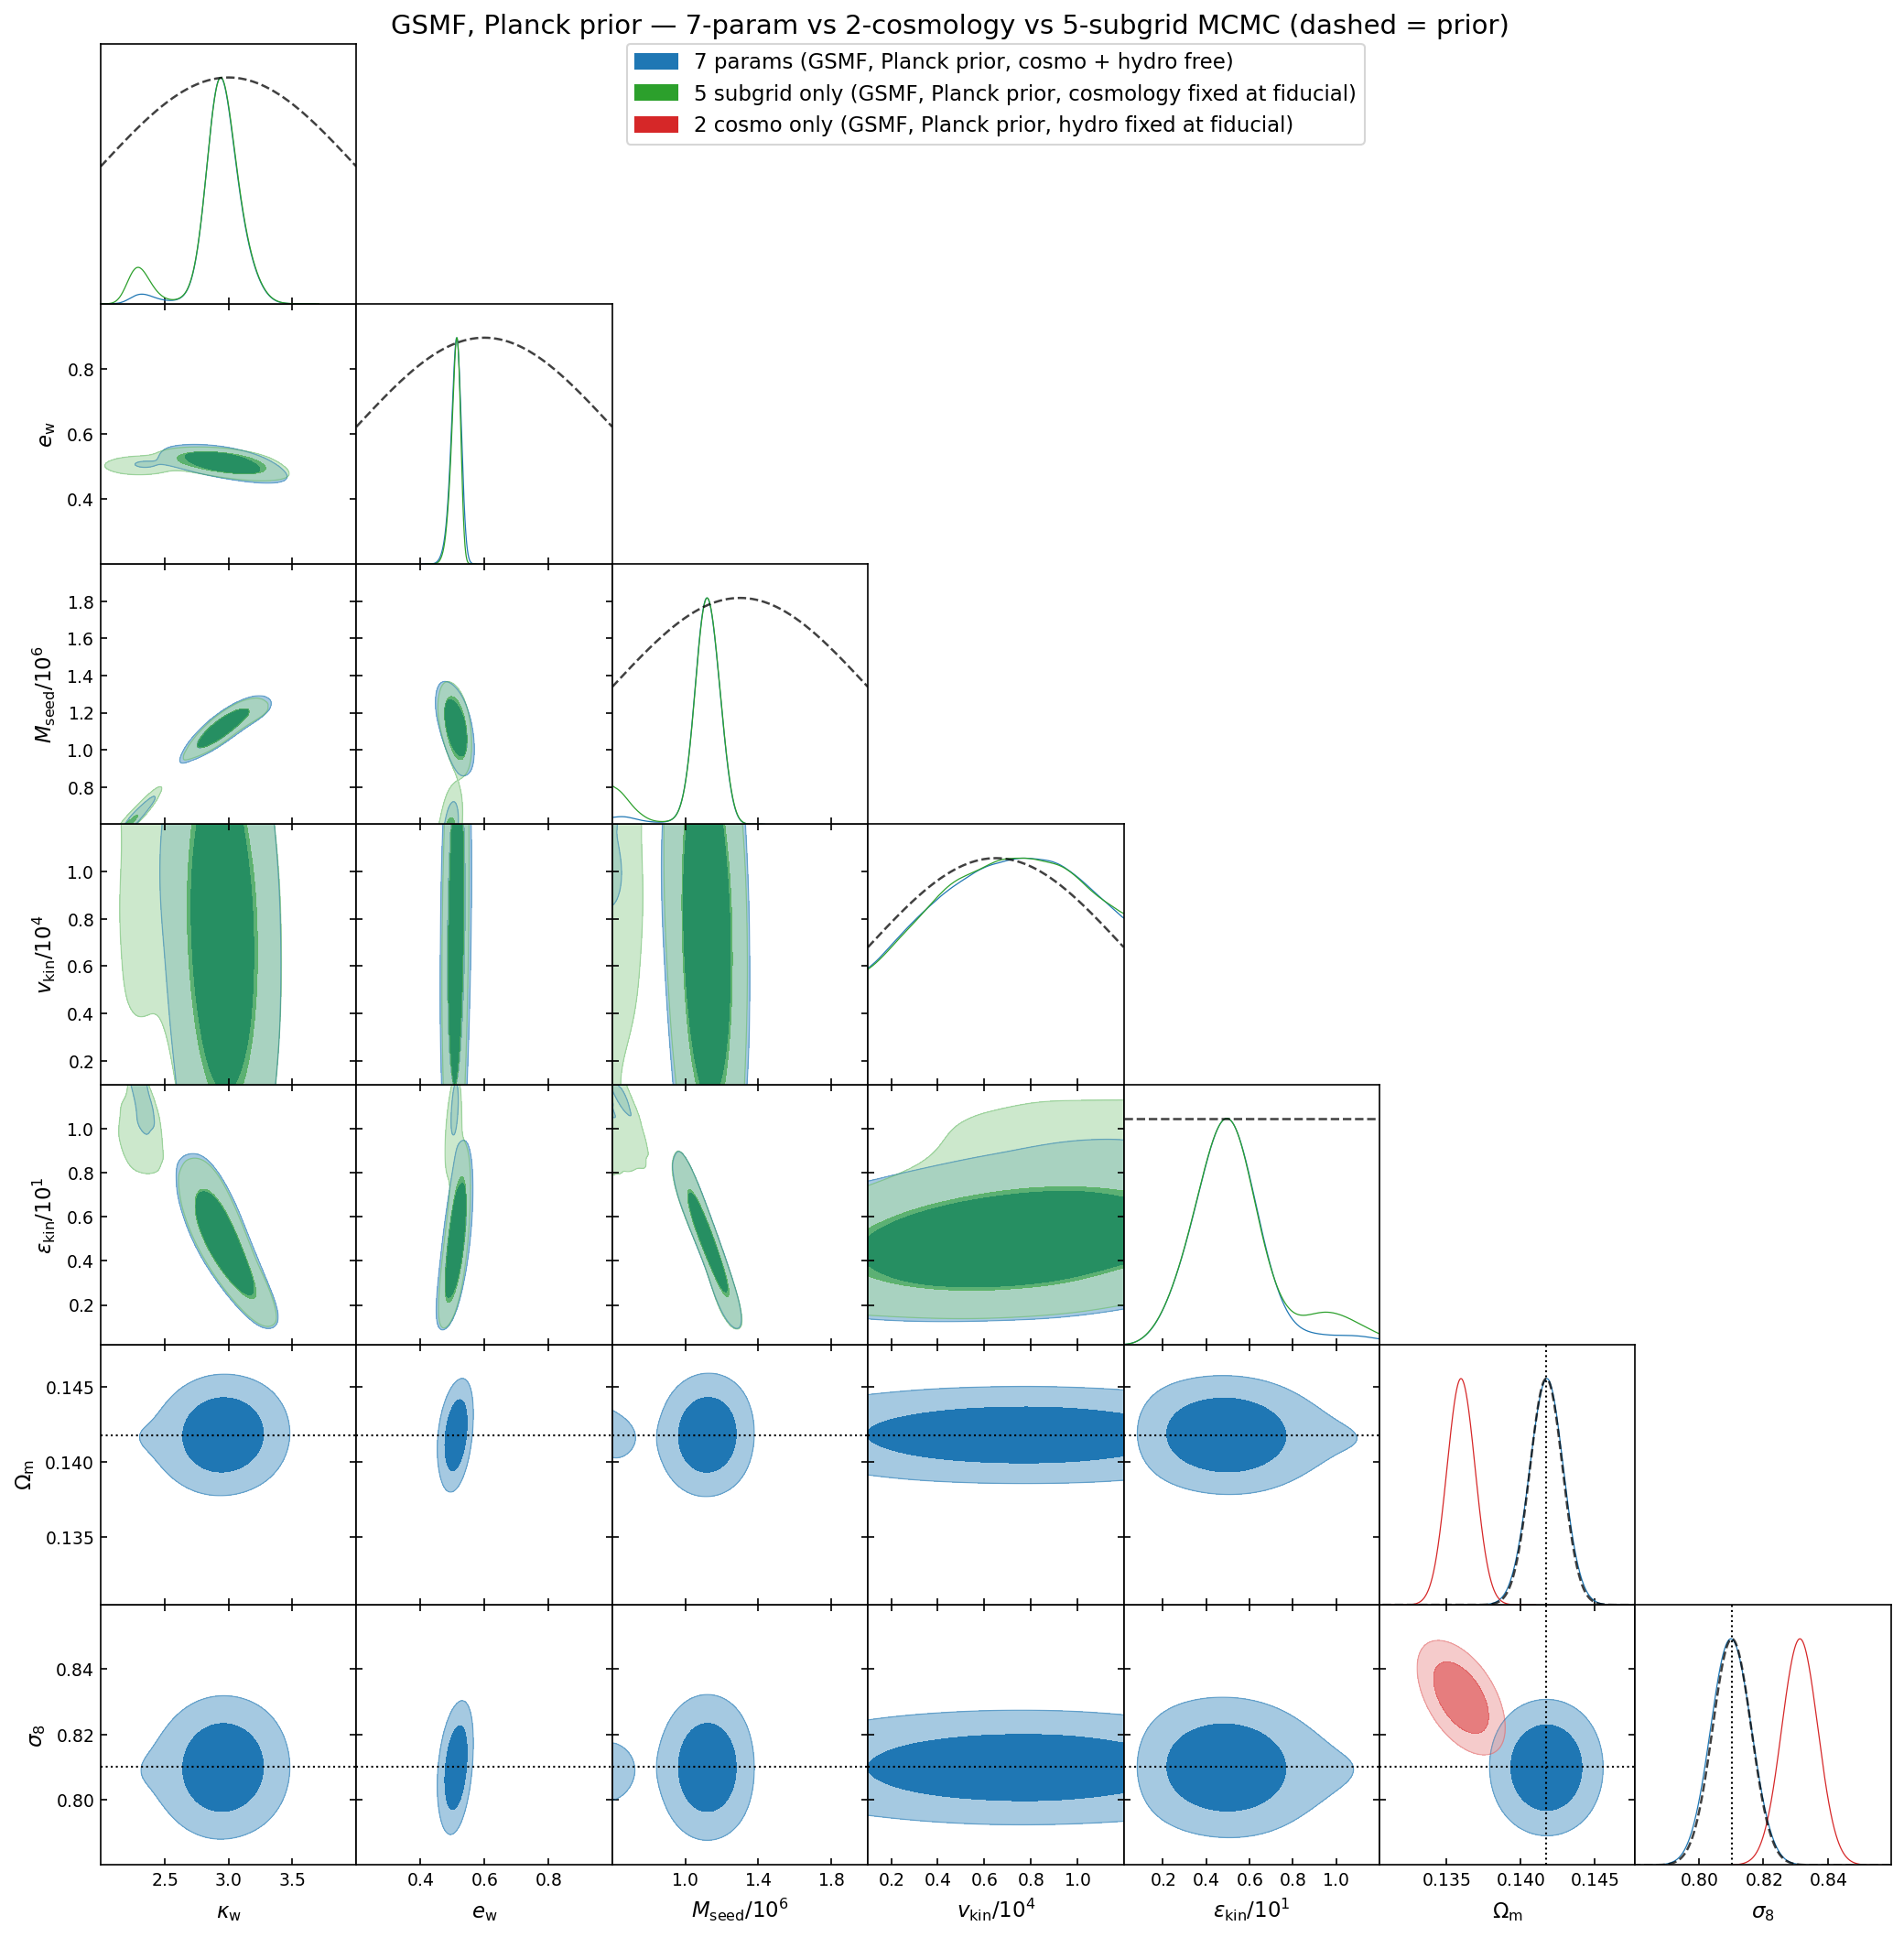
\includegraphics[width=1\linewidth]{plot_7p_vs_2cosmo_5subgrid_planck.png}
    \caption{GSMF-only, Planck prior. Three MCMC runs: all 7 parameters free
    (blue), 5 subgrid with cosmology fixed at fiducial (green), and 2 cosmology
    with subgrid fixed at fiducial (red). Priors are dashed. Under the Planck
    prior the 2-cosmology run no longer rails --- it forms a closed posterior
    (previously it was pushed to the $\omega_m$ box edge). The 7p and 5p subgrid
    contours overlap well.}
    \label{fig:2cosmo_gsmf}
\end{figure}

\begin{figure}[htbp]
    \centering
    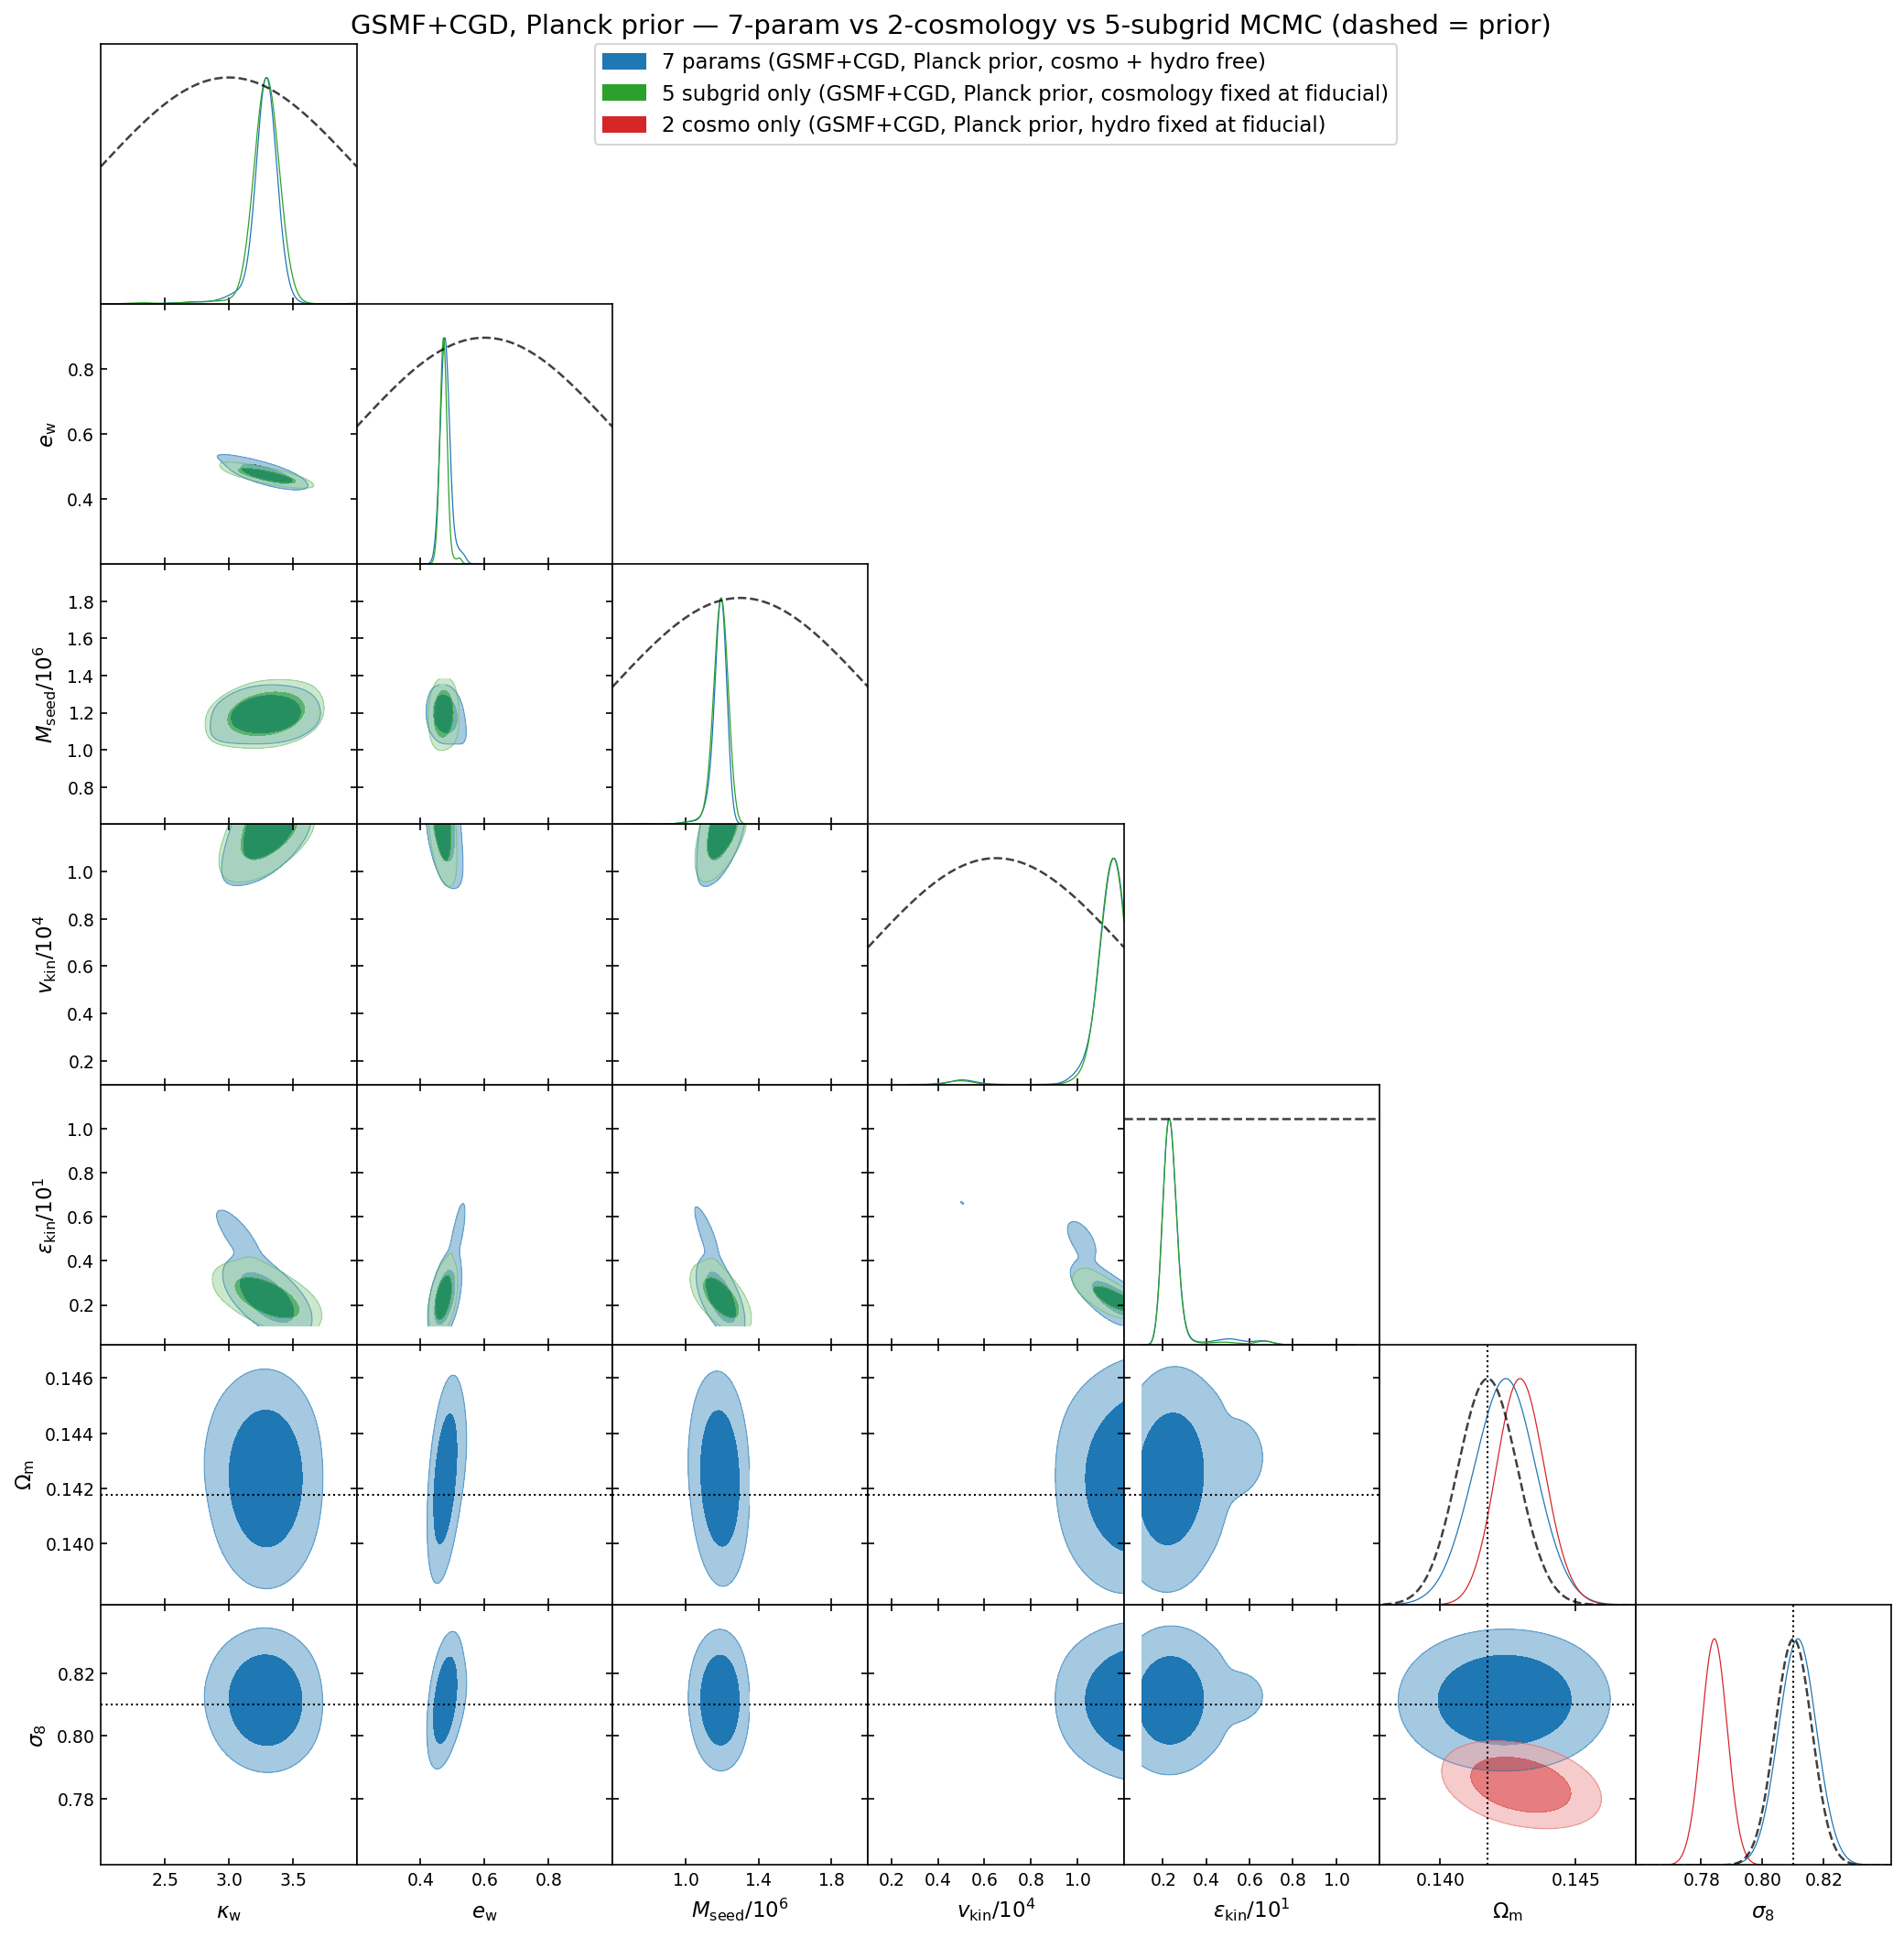
\includegraphics[width=1\linewidth]{plot_7p_vs_2cosmo_5subgrid_GSMF_CGD_planck.png}
    \caption{Same as Fig.~\ref{fig:2cosmo_gsmf} for GSMF$+$CGD. Again the Planck
    prior yields a closed 2-cosmology posterior. The fixed-hydro cosmology run
    (red) sits at slightly lower $\sigma_8$ than the marginalized 7p run,
    reflecting the residual $\sigma_8$ offset discussed above.}
    \label{fig:2cosmo_gsmf_cgd}
\end{figure}

\begin{figure}[htbp]
    \centering
    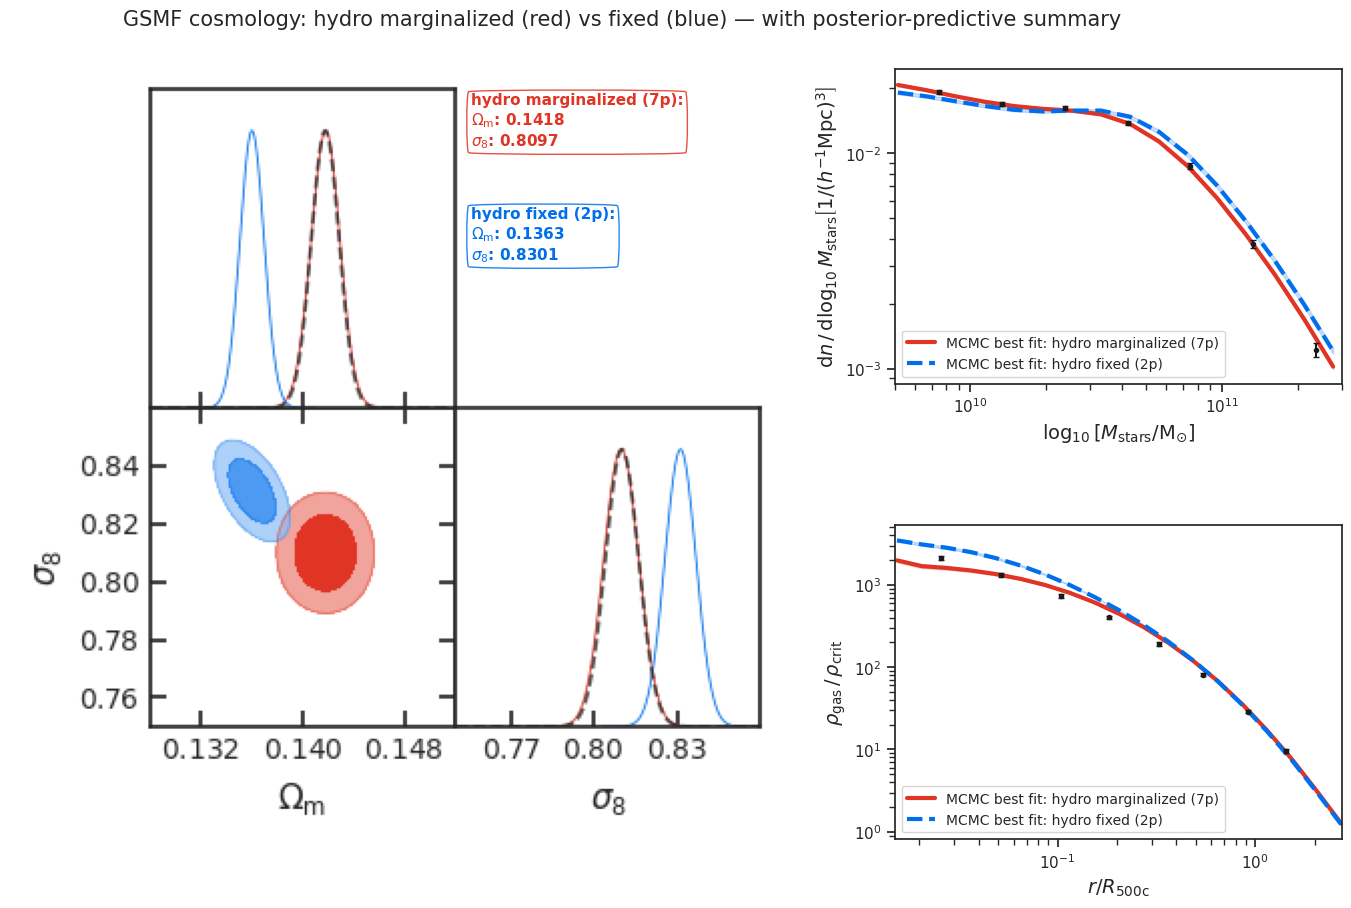
\includegraphics[width=1\linewidth]{plot_summary_planck_cosmo_marg_vs_fixed.png}
    \caption{GSMF, Planck prior --- effect of \emph{marginalizing over} vs.\
    \emph{fixing} the hydro parameters on the cosmology posterior, with the
    posterior-predictive summary. Red $=$ hydro marginalized (7p), blue $=$ hydro
    fixed at fiducial (2p). Both best fits reproduce the GSMF, but the fixed-hydro
    run reaches $\sigma_8=0.831$ (vs.\ $0.810$ marginalized) and lower $\omega_m$:
    fixing hydro biases and artificially tightens cosmology.}
    \label{fig:cosmo_margfix}
\end{figure}

\begin{figure}[htbp]
    \centering
    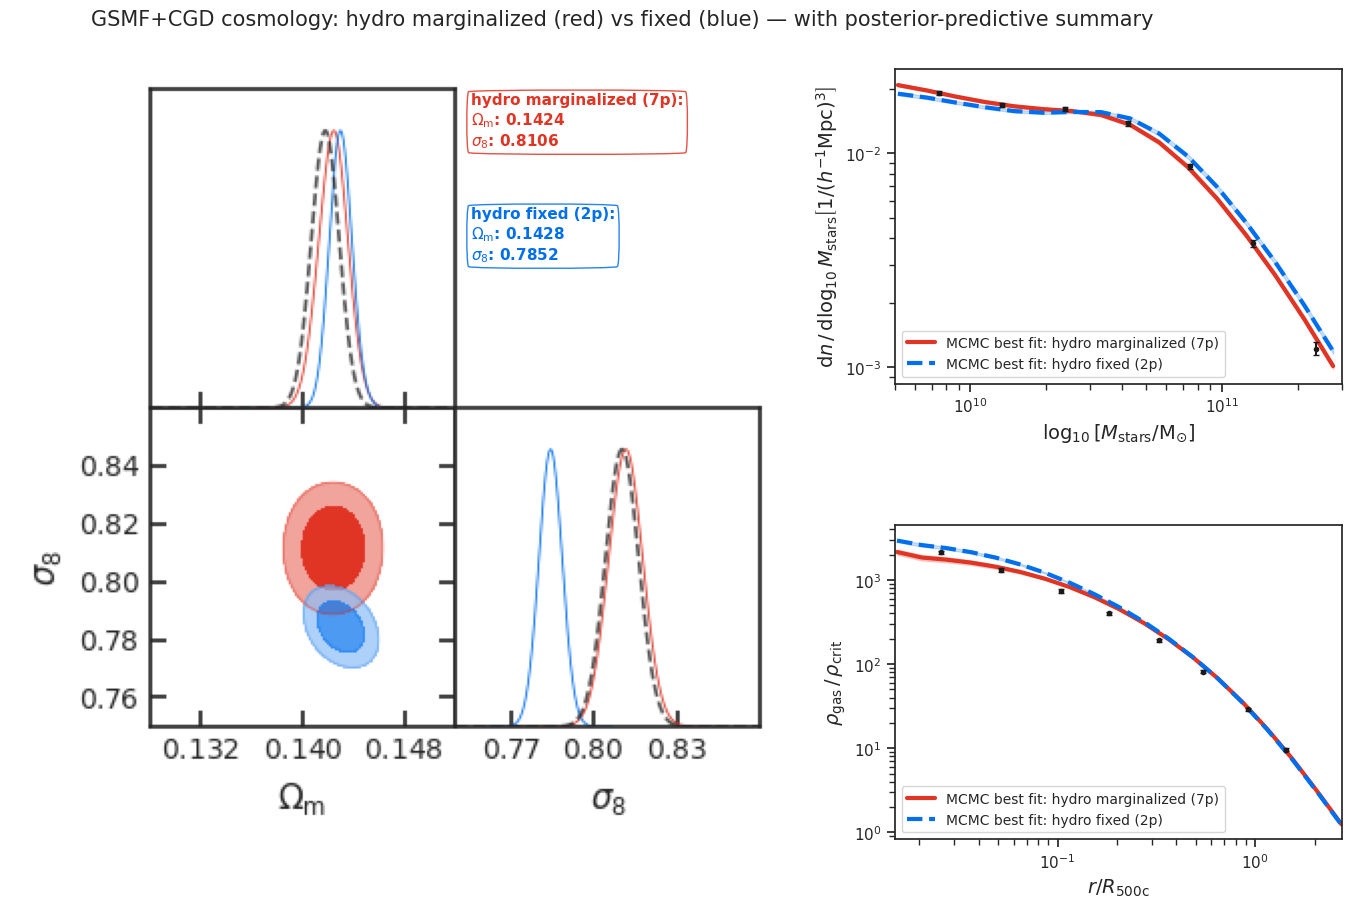
\includegraphics[width=1\linewidth]{plot_summary_planck_cosmo_marg_vs_fixed_GSMF_CGD.png}
    \caption{GSMF$+$CGD, Planck prior --- same test as
    Fig.~\ref{fig:cosmo_margfix}. Here fixing hydro pushes $\sigma_8$ \emph{low}
    ($0.785$ vs.\ $0.812$ marginalized). The right-hand panels show both best fits
    reproducing GSMF and CGD; the fixed-hydro fit trades cosmology to compensate
    for the pinned feedback, visible as a slight GSMF/CGD offset.}
    \label{fig:cosmo_margfix_cgd}
\end{figure}

\FloatBarrier

\section{Subgrid: marginalizing vs.\ fixing cosmology}

The mirror test: how much do the subgrid constraints move if cosmology is fixed
at fiducial rather than marginalized (both under the Planck prior)?

\begin{figure}[htbp]
    \centering
    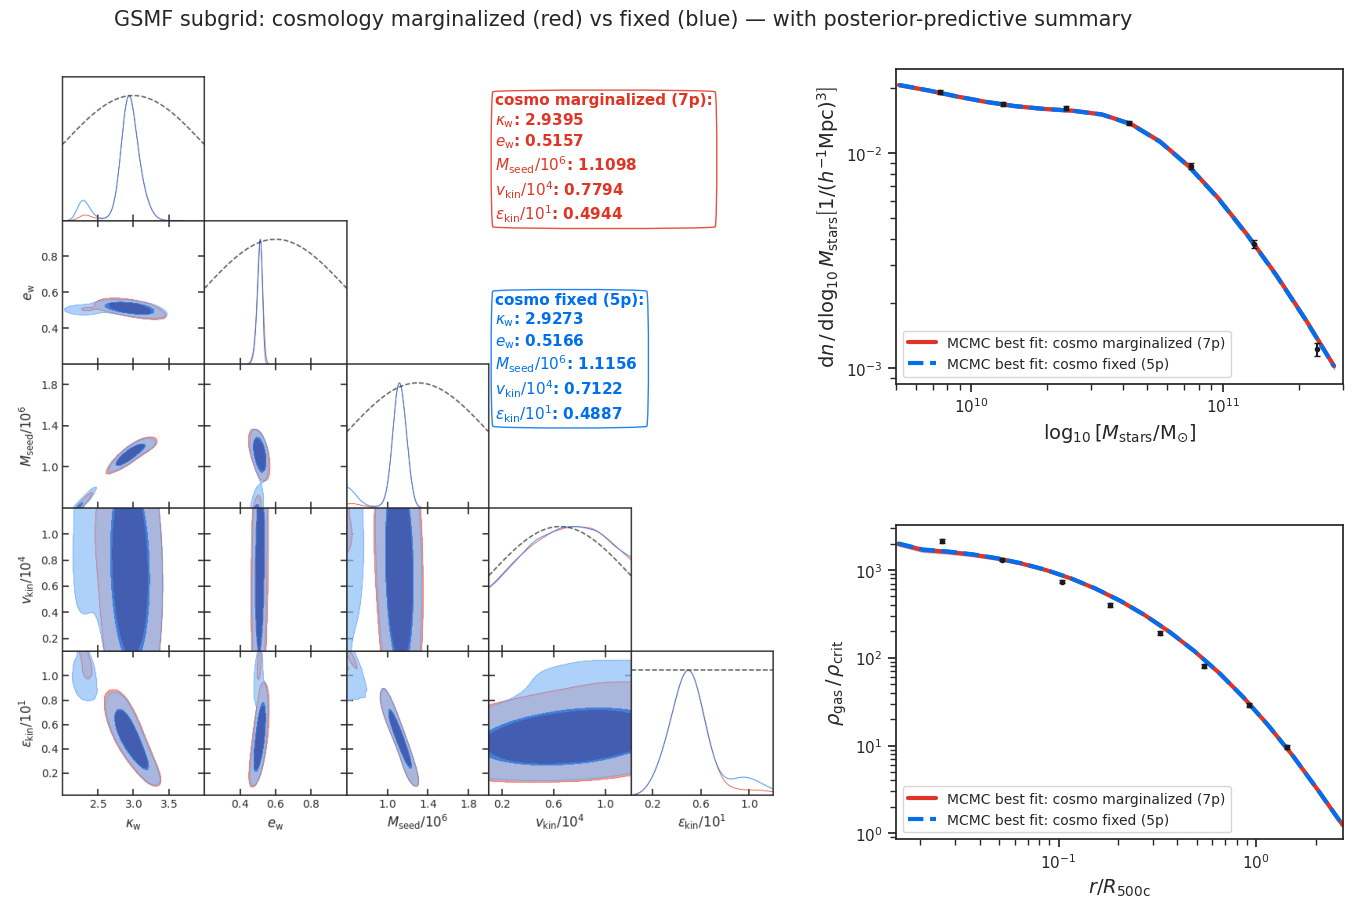
\includegraphics[width=1\linewidth]{plot_summary_planck_subgrid_marg_vs_fixed.png}
    \caption{GSMF: subgrid posteriors with cosmology marginalized (7p, red) vs.\
    fixed at fiducial (5p, blue), with the posterior-predictive summary. The
    subgrid modes are essentially unchanged and both best fits give the same GSMF
    prediction; fixing cosmology tightens $e_{\rm w}$ slightly, but the hydro
    constraints are largely insensitive to whether cosmology is marginalized.}
    \label{fig:subgrid_margfix}
\end{figure}

\begin{figure}[htbp]
    \centering
    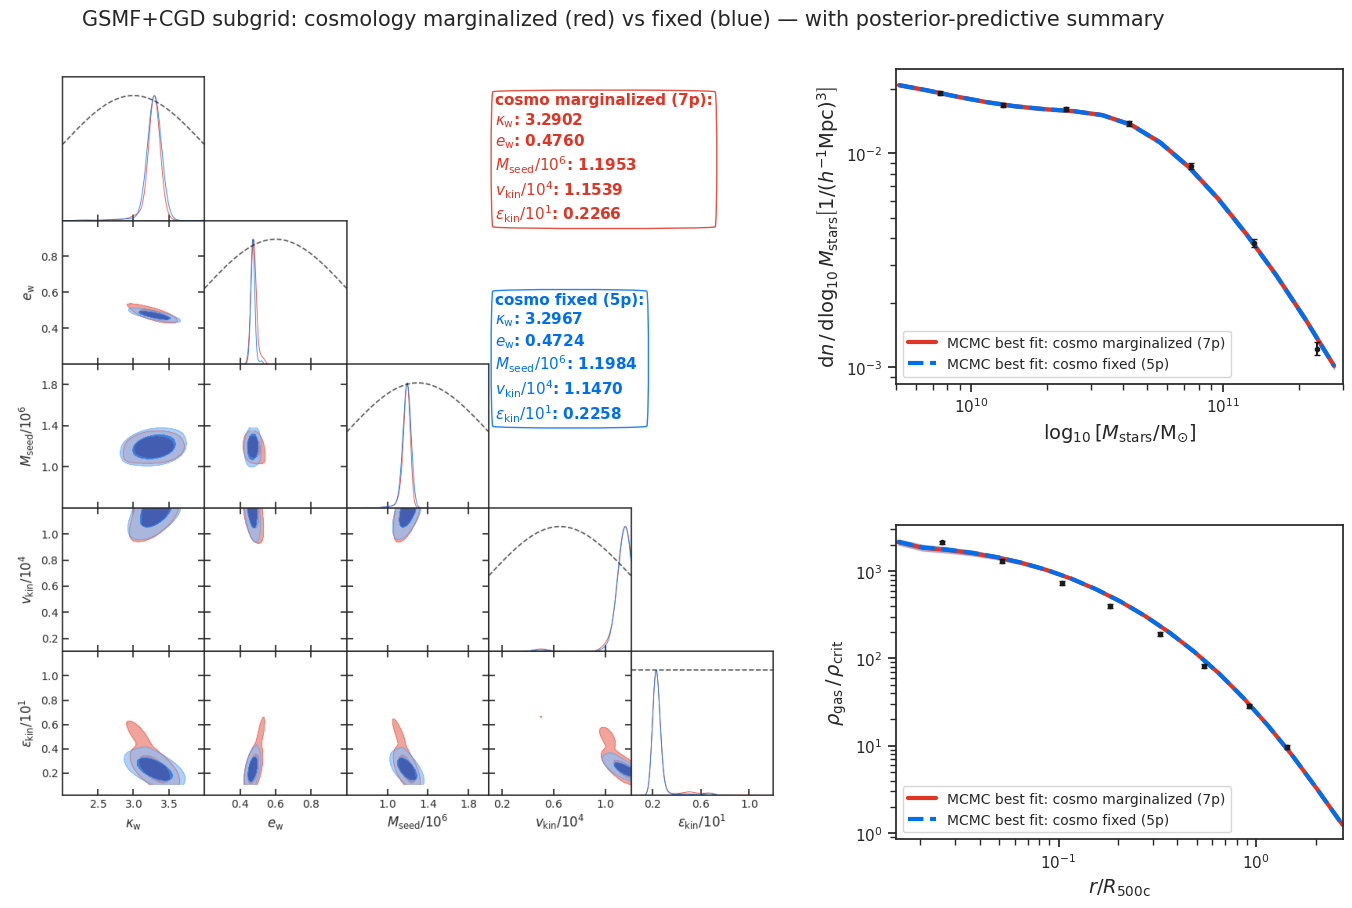
\includegraphics[width=1\linewidth]{plot_summary_planck_subgrid_marg_vs_fixed_GSMF_CGD.png}
    \caption{Same as Fig.~\ref{fig:subgrid_margfix} for GSMF$+$CGD. With CGD
    added, $v_{\rm kin}$ and $\epsilon_{\rm kin}$ are already tight; fixing
    cosmology produces only a marginal further tightening, and the GSMF/CGD
    predictions are indistinguishable.}
    \label{fig:subgrid_margfix_cgd}
\end{figure}

\begin{figure}[htbp]
    \centering
    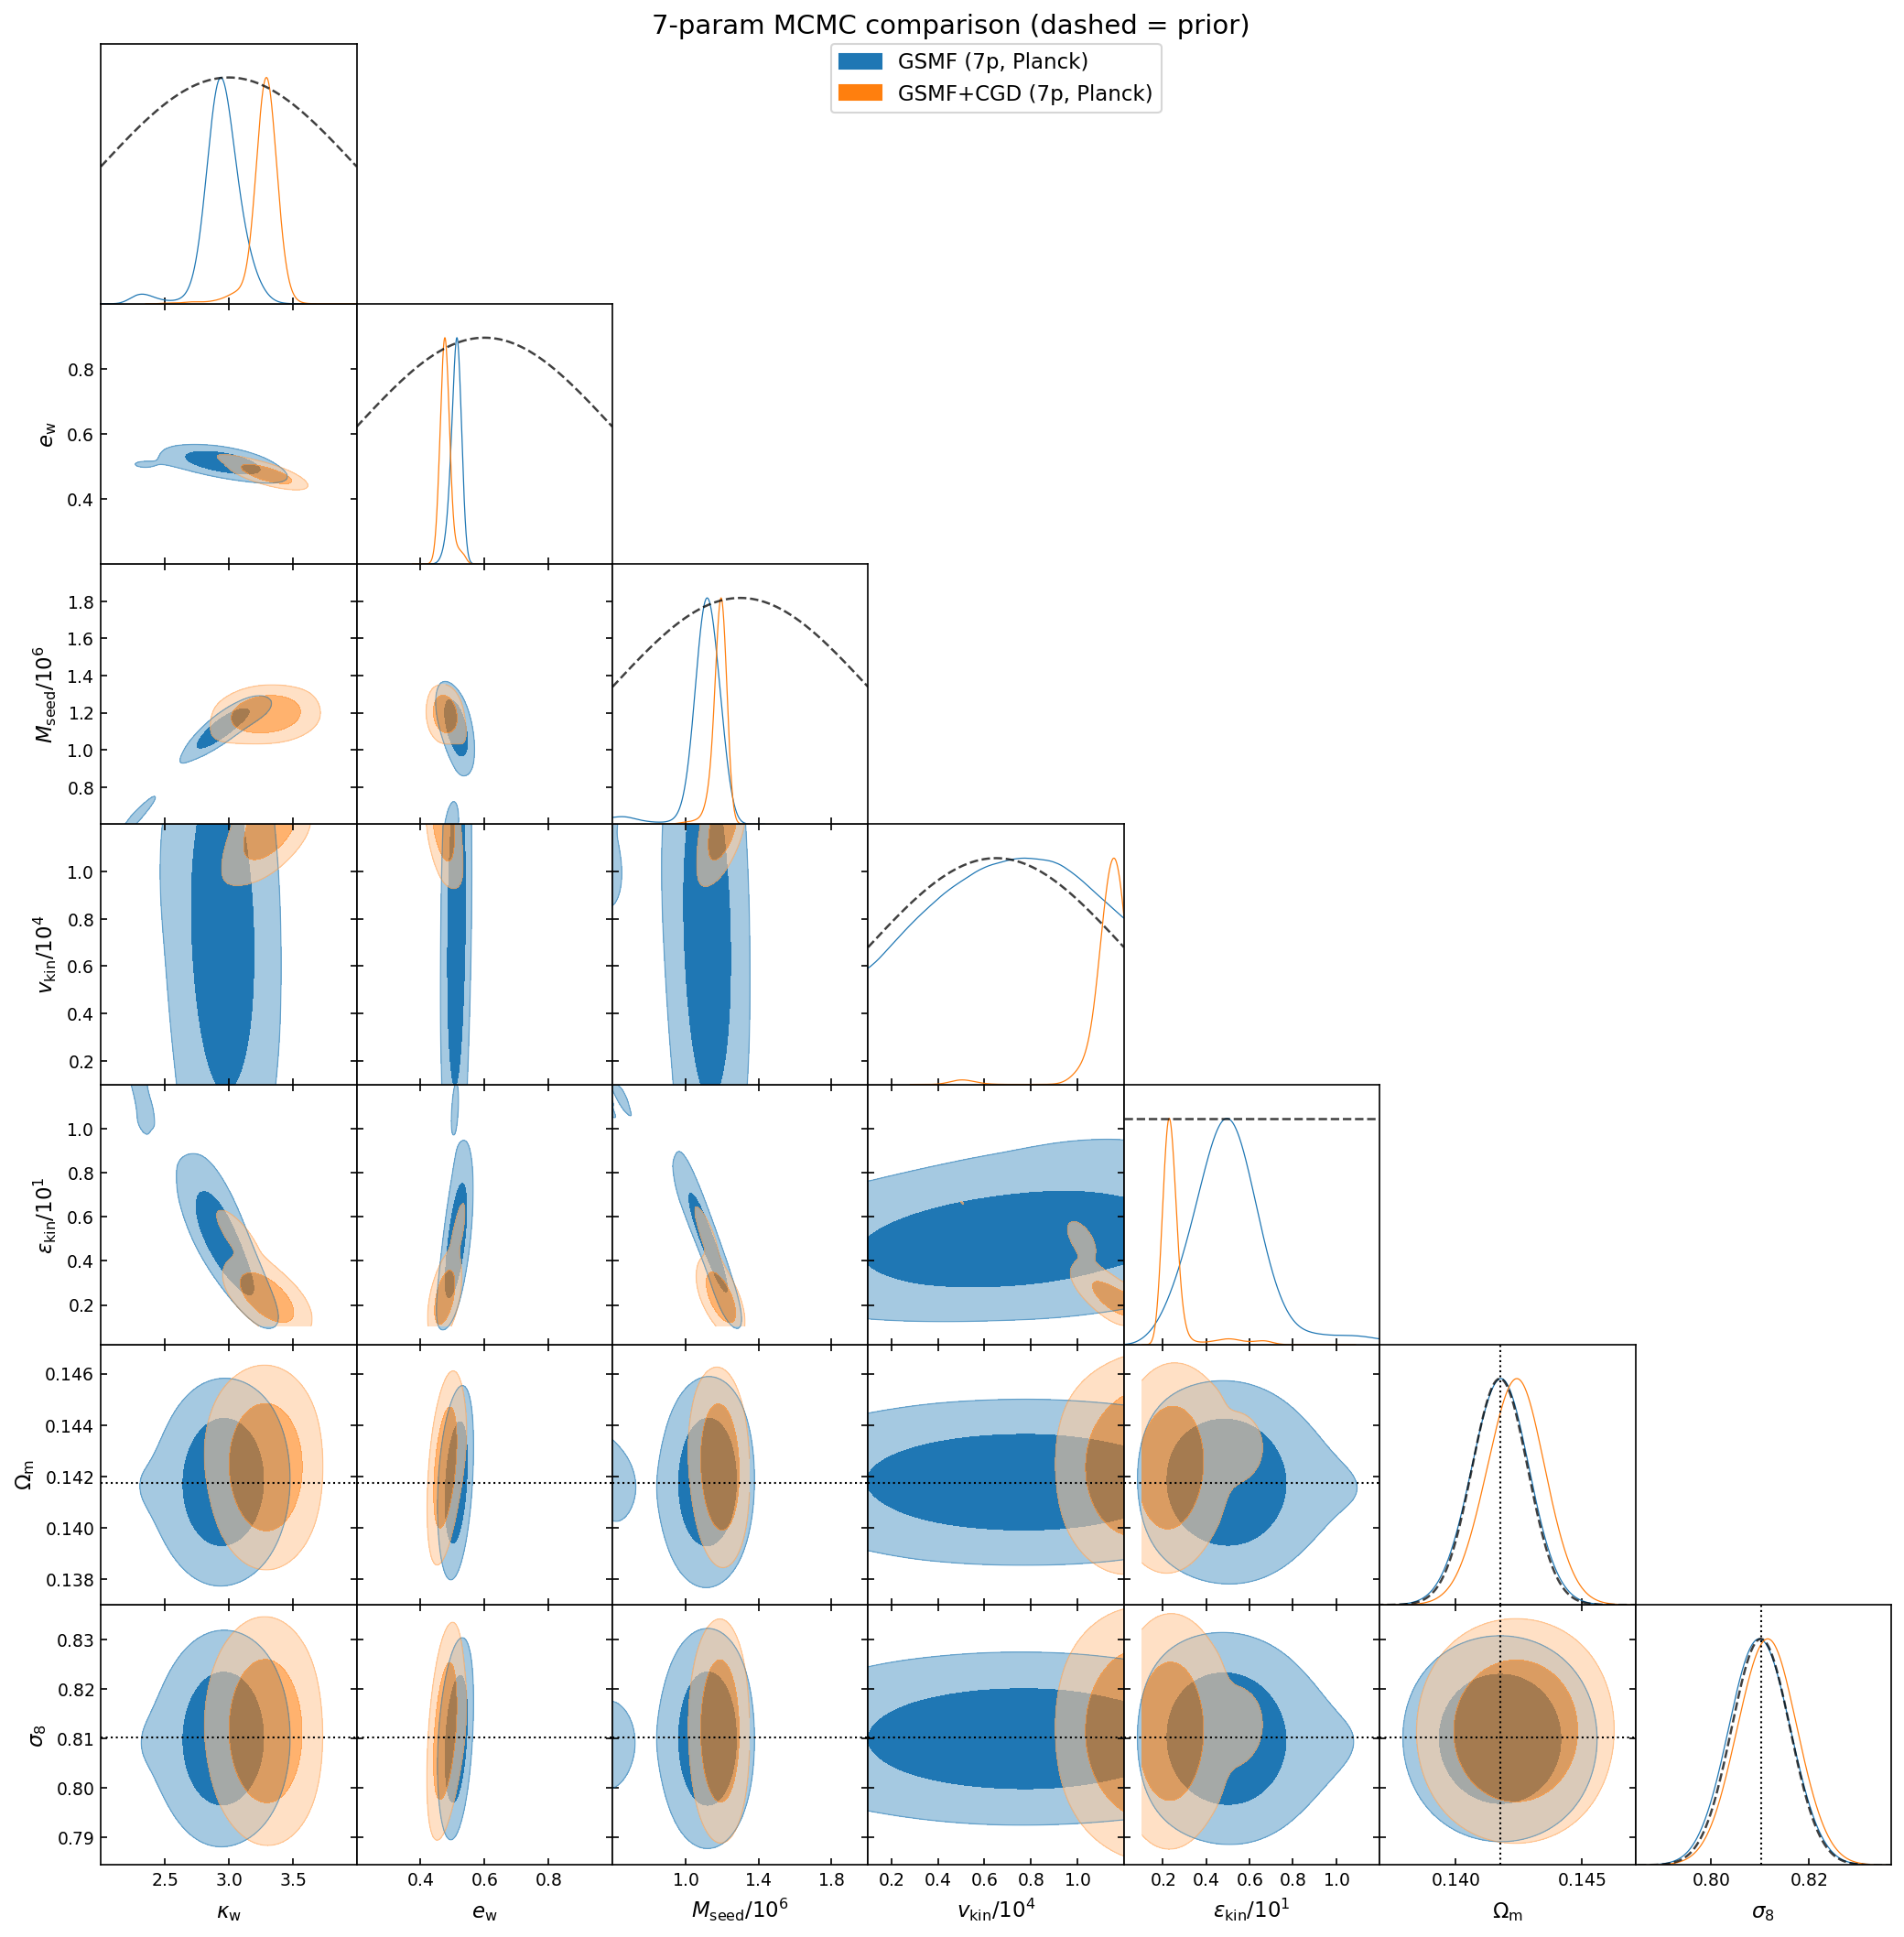
\includegraphics[width=1\linewidth]{plot_7p_GSMF_vs_GSMF_CGD_planck.png}
    \caption{Seven-parameter comparison of the two forward functions under the
    Planck prior: GSMF only (blue) vs.\ GSMF$+$CGD (orange). Priors dashed. Both
    now give closed cosmology posteriors consistent with fiducial; CGD's main
    effect is on the kinetic-feedback subgrid sector rather than on cosmology.}
    \label{fig:7p_compare}
\end{figure}

\FloatBarrier

\section{v1 $\leftrightarrow$ v2 (CosmoHydro) GSMF comparison}

The new (v2) pipeline is benchmarked against the legacy v1 inference on a
GSMF-only fit. Both pipelines fit the same Driver+2022 GSMF with mathematically
identical priors and likelihood; the difference is the simulation campaign
underneath (v1: 128\,Mpc HACC, 5p, fixed cosmology; v2: 400\,Mpc HAvoCC, 7p
design with cosmology varied). The v2 7p chain shown is \texttt{GSMF\_7p\_pk};
its subgrid marginals are prior-independent, so the comparison is unaffected by
the cosmology-prior update.

\begin{figure}[htbp]
    \centering
    
\includegraphics[width=1\linewidth]{corner_overlay.png}
    \caption{Triangle overlay of v1 (gray, 5p), v2 5p
    \texttt{GSMF\_5p\_fid\_cosmo} (blue, cosmology fixed at the project
    fiducial), and v2 7p \texttt{GSMF\_7p\_pk} (red, cosmology free). The shared
    subgrid axes are shown; contours are $1\sigma$ and $2\sigma$ filled. The two
    v2 fits agree on the four shared-range subgrid parameters; both show a small
    but consistent shift relative to v1 toward weaker AGN feedback, attributed to
    the different simulation campaign rather than to a pipeline change.}
    \label{fig:corner_overlay}
\end{figure}

\begin{figure}[htbp]
    \centering
    
\includegraphics[width=0.85\linewidth]{summary_stats_compare.png}
    \caption{Posterior-median emulator predictions overlaid on observations for
    GSMF, $f_{\rm gas}$, and CGD. Bands show the 16/84 percentile spread from
    posterior samples. All chains reproduce the observed GSMF amplitude within
    errors. CGD predictions diverge at small radius between the v1 and v2
    emulators, illustrating that the cluster-gas profile discriminates between
    simulation campaigns even when the GSMF constraint is identical.}
    \label{fig:summary_stats_compare}
\end{figure}

\paragraph{v1$\leftrightarrow$v2 posterior medians (scaled units).}

\begin{center}
\begin{tabular}{lccc}
\toprule
Parameter                 & v1    & v2 5p  & v2 7p \\
\midrule
$\kappa_{\rm w}$          & 3.144 & 2.936  & 2.946 \\
$e_{\rm w}$               & 0.495 & 0.512  & 0.512 \\
$M_{\rm seed}/10^6$       & 0.779 & 1.112  & 1.118 \\
$v_{\rm kin}/10^4$        & 0.682 & 0.690  & 0.691 \\
$\epsilon_{\rm kin}/10^1$ & 0.617 & 0.510  & 0.497 \\
$\omega_{\rm m}$          & --    & --     & 0.1418 \\
$\sigma_8$                & --    & --     & 0.8099 \\
\bottomrule
\end{tabular}
\end{center}

The v2 7p $\omega_{\rm m}=0.142$ and $\sigma_8=0.810$ (Planck prior) are
consistent with the project fiducial used by the 5p fit, again validating the
cosmology fix for subgrid-only calibrations.

\FloatBarrier

\section{Posterior summary}

\paragraph{Best-fit modes, Planck-prior 7p fits (scaled units).}

\begin{center}
\begin{tabular}{lcc}
\toprule
Parameter                 & \texttt{GSMF\_7p\_pk} & \texttt{GSMF\_CGD\_7p\_pk} \\
\midrule
$\kappa_{\rm w}$          & 2.940 & 3.290 \\
$e_{\rm w}$               & 0.516 & 0.476 \\
$M_{\rm seed}/10^6$       & 1.110 & 1.195 \\
$v_{\rm kin}/10^4$        & 0.779 & 1.154 \\
$\epsilon_{\rm kin}/10^1$ & 0.494 & 0.227 \\
$\omega_{\rm m}$          & 0.1418 & 0.1424 \\
$\sigma_8$                & 0.8097 & 0.8106 \\
\bottomrule
\end{tabular}
\end{center}

\paragraph{Cosmology: marginalized vs.\ fixed (median $\pm$ std).}

\begin{center}
\begin{tabular}{lcccc}
\toprule
 & \multicolumn{2}{c}{GSMF} & \multicolumn{2}{c}{GSMF$+$CGD} \\
\cmidrule(lr){2-3}\cmidrule(lr){4-5}
 & 7p (marg.) & 2p (fixed) & 7p (marg.) & 2p (fixed) \\
\midrule
$\omega_{\rm m}$ & $0.1418\pm0.0011$ & $0.1360\pm0.0009$ & $0.1424\pm0.0011$ & $0.1430\pm0.0009$ \\
$\sigma_8$       & $0.810\pm0.006$   & $0.831\pm0.005$   & $0.812\pm0.006$   & $0.784\pm0.004$ \\
\bottomrule
\end{tabular}
\end{center}

The marginalized cosmology posteriors sit on the project fiducial
($\omega_m\!=\!0.142$, $\sigma_8\!=\!0.810$), validating the choice of cosmology
fix for subgrid-only calibrations. Fixing hydro instead biases $\sigma_8$ (high
for GSMF, low for GSMF$+$CGD) and artificially shrinks the error bar --- the
apparent precision gain is spurious, a consequence of breaking the
hydro$\leftrightarrow$cosmology degeneracy.

\FloatBarrier

\section{To-do}

\begin{itemize}
  \item Multi-$z$ GSMF MCMC, exploiting the redshift-aware emulators
        from training notebook 02. The likelihood scaffolding already
        supports per-snapshot likelihoods; the trial config is the
        next planned addition.
  \item Cluster-profile-only calibration
        (\texttt{CGD\_CGED\_cluster}) with cosmology fixed at the
        project fiducial, to isolate the subgrid information in
        cluster-scale baryonic observables.
  \item Joint $P(k)$ + cluster constraints: with the suppression
        emulator validated, the $P(k)$ likelihood can be combined with
        $f_{\rm gas}$ for an independent baryonic-feedback handle.
  \item Follow up the residual $\sigma_8$ offset seen when hydro is fixed
        (GSMF$+$CGD prefers $\sigma_8\!\approx\!0.784$): is it a genuine
        data-model tension or a fixed-hydro artefact? The marginalized 7p
        fit resolving to fiducial suggests the latter.
  \item Identify probes that calibrate cosmology without being strongly
        affected by subgrid, and vice versa.
  \item Constrain cosmology from low-$k$ $P(k)$, then use those calibrations
        as priors for subgrid calibration (avoiding circularity).
\end{itemize}

\end{document}
